\RequirePackage[l2tabu, orthodox,abort]{nag}

\InputIfFileExists{jfsettings}{}{
\documentclass[12pt,oneside,reqno]{amsart}
\usepackage[a4paper,portrait,left=1.5cm,outer=3.5cm,headheight=15pt,bottom=3cm,top=3cm]{geometry} 
}

%%%%%%%%%%%%%%%%%%%%%%%%%%%%%%%%%%%%%%%%%%%%%%%%%%%%%%%%%%%%%%%&
% Draft settings
\usepackage{xcolor}
\usepackage[color]{showkeys}
\definecolor{refkey}{rgb}{0.3,0.5,0.3}
\definecolor{labelkey}{rgb}{0.3,0.5,0.3}
\definecolor{todo}{rgb}{0.6,0.9,0.5}
\usepackage[textwidth=3cm,textsize=tiny,color=todo]{todonotes}


%%%%%%%%%%%%%%%%%%%%%%%%%%%%%%%%%%%%%%%%%%%%%%%%%%%%%%%%%%%%%%%%%
%%  GENERAL SETTINGS

\usepackage{amsmath,amssymb,amsfonts,amsthm} % ams stuff everywhere
\usepackage{array}                 % math in tabular etc.
\usepackage{booktabs}              % improve table rendering
\usepackage[utf8]{inputenc}        % UTF8 fonts
\usepackage[T1]{fontenc}           % Fix font encoding issues with accented chars
\usepackage[english]{babel}        % Language awareness
\usepackage{csquotes}              % Context sensitive qouting
\usepackage{enumitem}              % no dull items
\usepackage{tikz}
\usepackage{verbatim}
\usepackage{graphicx}
\usepackage{fouriernc}
\usepackage[amssymb,thickspace,thinqspace]{SIunits}

\graphicspath{ {./} {./pic/}}
\numberwithin{equation}{section}




\title[Verification of Butler-Volmer derivation]{Numerical verification of the derivation of the Butler-Volmer equation from
the Nernst-Planck equations\\ Draft}
\author{$\dots$}
\date{\today}



\begin{document}
\maketitle

\section{Introduction}

The authors of \cite{dreyer2016new} provides a thermodynamically and  mathematically motivated  derivation of
Butler-Volmer - like  equations assuming that 
\begin{itemize}
\item all reactions take place at the interface between the electrolyte
and the metal (interface I)
\item in a boundary layer defined by the plane of zero charge, short relaxation
  times allow the assumption that the electrochemical potential of the dissolved species
  is constant
\end{itemize}
A similar analysis already was performed in \cite{rubinstein1990electro}, albeit without the
connection to the Butler-Volmer equation.

This paper attempts to provide  an assessment of this derivation using
numerical    computations   based    on   Nernst-Planck-Poisson    and
Nernst-Planck-Ohm systems.

%%%%%%%%%%%%%%%%%%%%%%%%%%%%%%%%%%%%%%%%%%%%%%%%%%%%%%%%%%%%
%%%%%%%%%%%%%%%%%%%%%%%%%%%%%%%%%%%%%%%%%%%%%%%%%%%%%%%%%%%%
\section{Electrolyte models}

In this  section, we  introduce three  electrolyte models  and discuss
their boundary conditions and their interconnections. For the notations,
see table \ref{tab:notations}.

%%%%%%%%%%%%%%%%%%%%%%%%%%%%%%%%%%%%%%%%%%%%%%%%%%%%%%%%%%%%
\subsection{Nernst-Planck-Poisson  with  volume constraints in mechanical equilibrium} 
\cite{dreyer2014mixture,fuhrmann2016numerical,dreyer2017new, springer}
\begin{subequations}\label{sys:PNP}
\begin{align}
  -\nabla \varepsilon \nabla \phi&= q\\
  \partial_t c_i  + \nabla \cdot \mathbf N_i  &=0 & (i=1\dots N)\\
  \mathbf N_i &= - \frac{D_i}{RT} c_i \left( \nabla \mu_i -m_i\nabla \mu_0 + z_i F \nabla \phi \right)& (i=1\dots N). \label{eq:NP}
\end{align}

From the momentum balance at zero barycentric velocity, the pressure $p$ obeys the relationship $\nabla p = q \nabla \phi$
which under mechanical equilibrium conditions is replaced \cite{Fuhrmann2015} by :
\begin{align}
  -\Delta p + \nabla \cdot q \nabla \phi \label{eq:press}
\end{align}
The system is closed by the incompressibility condition
\begin{align}\label{eq:incompress}
  \sum_{i=0}^N \bar v_ic_i&=1
\end{align}
and the relationship between chemical potentials and concentrations \cite{dreyer2013overcoming} :
\begin{align}\label{eq:constrel}
  \mu_i &= \mu_i^\circ + \bar v_i(p-p^\circ) + RT \ln \frac{c_i}{\bar c}.  & (i=0\dots N)
\end{align}
\end{subequations}


By \eqref{eq:incompress} one can obtain the solvent concentration $c_0$  from the solute concentrations
$c_1\dots c_N$:
\begin{align}
  \label{eq:c0}
  c_0&=\frac{1}{v_0} -  \sum_{i=1}^N  \frac{\bar v_i}{v_0}c_i
\end{align}
The diffusive mass fluxes are defined relative to the barycentric velocity \cite{dreyer2013overcoming,Fuhrmann2015} which is assumed to be zero:
\begin{align}
  \sum_{i=0}^N M_i\mathbf N_i&=0
\end{align}

\begin{comment}
  
m= RTlog(v c)
v*c =exp(mu/(RT))
c= exp(mu/(RT))/v

nabla c = 1/RT exp(mu/(RT))/v \nabla mu = 1/RT c \nabla mu
\nabla mu = RT nabla log(c) + RT nabla log(v) = RT nabla log(c)
\end{comment}

For the derivation of the numerical scheme we define the \textit{excess chemical potential}
\begin{align}\label{eq:muexdef}
  \mu^{ex}_i = \mu_i - m_i\mu_0 -  RT \log \frac{c_i}{c_{ref}}
\end{align}
where $c_{ref}$ is some constant reference concentration. Here, we choose $c_{ref}=\frac{1}{v_0}$, the
concentration of the solvent without ion content.

This   allows to rewrite the Nernst-Planck flux as 
\begin{align}
  N_i &=-\frac{D}{RT} c_i \nabla\left( RT \log (v_0c_i)  +  \mu^i_{ex} +z_iF\nabla\phi\right) \nonumber\\
      &= .D\nabla c_i  -  c_i\frac{D_i}{RT}(\nabla\mu^i_{ex} +z_iF\nabla\phi) \label{eq:flux}
\end{align}
The generalized drift-diffusion representation \eqref{eq:flux} will allow to apply the excess chemical potential
scheme (SEDAN scheme) \cite{GaudeulFuhrmann, EisenbergLiu} which has been shown to be thermodynamically correct and convergent in the case without pressure
dependency. As we will take the gradient of it, the constant parts depending on $\mu_i^\circ$ and $p^\circ$ can be
omitted from the calculation.

For $i=1\dots N$ we have
\begin{align}
  \mu_i^{ex} &= \mu_i -m_i \mu_0  - RT \log (v_0c_i)\nonumber\\
             &= \bar v_ip +  RT \log \frac{c_i}{\bar c}  -m_i\left(  v_0p + RT \log \frac{c_0}{\bar c}\right)  - RT \log (v_0c_i)  \nonumber\\
            &= \bar v_ip - RT\log v_0\bar c -m_i\left(v_0p + RT \log \frac{c_0}{\bar c}\right)\nonumber\\
            &= \left(\bar v_i-m_iv_0\right)p -m_iRT\log \frac{c_0}{\bar c} - RT\log v_0 \bar c \label{eq:muex}
\end{align}
and express $c_0$ via \eqref{eq:c0} and $\bar c$ in terms of $c_1\dots c_N$:
\begin{align*}
  \bar c &% = \frac{1}{v_0} -  \sum_{i=1}^N \frac{\bar v_i}{v_0}c_i + \sum_{i=1}^N  c_i
          = \frac{1}{v_0} + \sum_{i=1}^N \left(1- \frac{\bar v_i}{v_0}\right) c_i .
\end{align*}

\newpage
The dependency $\mu_i^{ex}=\mu_i^{ex}(c_1\dots c_N, p)$  encodes the non-ideality properties of the mixture.
The excess chemical potential is linked to the \textit{activity coefficient} $\gamma_i=\exp(-\frac{\mu_i^{ex}}{RT})$
\cite{IUPAC,Fuhrmann2015}
\begin{align}
  \gamma_i&=\exp(-\frac{\mu_i^{ex}}{RT})\\
         &= \frac{1}{v_0\bar c}\exp\left(\frac{\bar v_i-m_iv_0}{RT}p\right)\left(\frac{\bar c}{c_0}\right)^{m_i} \label{eq:gamma}
\end{align}

There are some noteworthy special cases.

\subsubsection{BAO Model}
\cite{Borukhov, Andelman, Orland, RingeEtAl}
\begin{align}
  \gamma = \frac{1}{1-\sum_{i=1}^N v_i c_i} \label{eq:BAO}
\end{align}
with $v_\alpha = N_A (a_\alpha^{cell})^3$. Under the assumption that $\kappa_i=0$, this gives
$\gamma_i = \frac{1}{v_0 c_0}$. Assuming $m_i=1, \kappa_i=0$  (equal species molar masses),  
\eqref{eq:gamma} turns into
\begin{align}
  \gamma_i
         &= \frac{1}{v_0c_0}\exp\left(\frac{v_i-v_0}{RT}p\right),
\end{align}
and one sees that the model \eqref{eq:BAO} misses the influence of the pressure on the
activity coefficient and thus the chemical excess potential.


\subsubsection{BF Model}
\cite{Fuhrmann2015}
Set $v_i=v_0$, $M_i=M_0$, $\kappa_i=0$. Thus $m_i=1$, $\bar v_i=v_i$, $\bar v_i -m_i v_0=0$.
As a consequence, $\mu_i^{ex} = -RT\log c_0$, and notably it is independent of $p$.
Also, $\bar c=\frac{1}{v_0}$ and $c_0=\frac{1}{v_0} - \sum c_i$.



\clearpage
\subsubsection{Constant density (Springer paper)}!!!


\subsection{Equilibrium problem}
\eqref{eq:flux} gives
\begin{align}\label{eq:fluxx}
  \mathbf N_i &= - D_i\frac{c_i}{RT}\nabla\left( \mu_i +  \mu_i^{ex} + z_i F \nabla \phi \right)
\end{align}
Zero flux gives (by interpreting the integration constant as the log of a bulk concentration):
\begin{align}
  \mu_i   &=   - \mu_i^{ex} - z_i F \nabla \phi + \text{const}\\
  c_i   &=  c_i^{bulk}\exp\left( -\frac{\mu_i^{ex} + z_i F \nabla \phi}{RT}\right) 
\end{align}


\begin{table}
  \begin{tabular}{rl}
    $\phi $ &electrostatic potential\\
    $p$ & pressure\\
    $\mu_i$& species chemical potential\\
    $c_i$& species molar concentration\\
    $  \bar c = \sum_{i=0}^N  c_i$& molar concentration of mixture\\
    $N_i$& species molar flux\\
    $p^\circ$ & reference pressure\\
    $\mu_i^\circ$& species reference chemical potential\\
    $v_i$ & species molar volume\\ 
    $M_i$ & species molar mass\\
    $\kappa_i$ & species solvation number\\
    $z_i$ & species charge number\\
    $\varepsilon$& dielectric constant\\
    $F$ & Faraday constant\\
    $R$ & Molar gas constant\\
    $T$ & Temperature\\
    $q=F\sum_{i=1}^N z_i c_i$ & Electric charge density\\
    $\bar v_i = v_i + \kappa_i v_0$ & solvated molar volume\\
    $m_i=\frac{M_i+\kappa_i M_0}{M_0}=\frac{M_i}{M_0}+\kappa_i$ & Solvated molar mass ratio
  \end{tabular}
  \medskip
  
  \caption{Notations}
  \label{tab:notations}
\end{table}

%%%%%%%%%%%%%%%%%%%%%%%%%%%%%%%%%%%%%%%%%%%%%%%%%%%%%%%%%%%%%%%%%%%%%%%%%%%%%%%%%%%%%%%%%%%%%%%%
\subsection{Flux discretization}
Implicit Euler Voronoi finite volumes with modified Scharfetter Gummel fluxes
$\equiv$ upwinding by exponential fitting
!!! replace n!
Let $\delta\mu^{ex,n}_{i,KL}=\frac{1}{D_iRT}(\mu^{ex,n}_{i,K}-\mu^{ex,n}_{i,L})$, $\delta\phi^n_{KL}= \frac{F}{D_iRT}(\phi^n_K-\phi^n_L)$, $B(x)=\frac{x}{e^x-1}$

\begin{figure}
  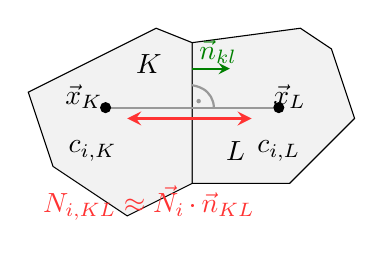
\begin{tikzpicture}[scale=0.55,>=stealth,shorten >=2pt]
    % \draw[step=1cm] (-4,-4) grid (8,4);
    \filldraw[fill=gray!10, draw=black] 
    (2,1.5) -- 
    (4.5,1.83333) -- 
    (5.21429,1.35714) -- 
    (5.75,-0.25) -- 
    (4.25,-1.75) -- 
    (2,-1.75) -- 
    cycle;
    \filldraw[fill=gray!10, draw=black] 
    (2,1.5) -- 
    (1.16667,1.83333) -- 
    (-1.78571,0.357143) -- 
    (-1.21429,-1.35714) -- 
    (0.5,-2.5) -- 
    (2,-1.75) -- 
    cycle;
    
    \draw[thick,gray!80] (0,0) -- (4,0);
    
    \draw (0,0) node[inner sep=0.5mm,shape=circle,fill] {} ;
    \draw (4,0) node[inner sep=0.5mm,shape=circle,fill] {} ;
    
    
    \draw (-0.5,0.25) node {$\vec{x}_K$};
    \draw (-0.3,-1) node {$c_{i,K}$};
    
    
    \draw (4.25,0.25) node {$\vec{x}_L$};
    \draw (4.0,-1) node {$c_{i,L}$};
    \draw[very thick,red!80,<->] (0.5,-0.25) -- (3.5,-0.25);
    \draw (1,-2.2) node {\textcolor{red!80}{$N_{i,KL}\approx \vec{N_i}\cdot\vec{n}_{KL} $}};
    
    
    % \draw (2.4,0.9) node {$\sigma_{kl}$};
    
    \draw (1,1) node {$K$};
    \draw (3,-1) node {$L$};
    
    % \draw[thick,black,->] (1,-0.2) -- (3,-0.2);
    % \draw(1.5,-0.55) node {$\textcolor{black}{j_{k\ell}}$};
    
    \draw[green!50!black,thick,->] (2,0.9) -- (3,0.9);
    \draw(2.6,1.3) node {$\textcolor{green!50!black}{\vec{n}_{kl}}$};
    \draw [thick, gray!80] (2.5,0) arc (0:105:0.5);
    \draw (2.15,0.15) node[thick,gray!80,inner sep=0.2mm,shape=circle,fill] {};
  \end{tikzpicture}
  \caption{!!!}
\end{figure}

    
    \begin{itemize}
    \item Discrete Poisson
      \begin{align*}
        0&=-\sum\limits_{L\; \text{neighbor of}\; K} |\partial K\cap\partial L| E^n_{KL} + |K|F\sum_{i=1}^N z_i c^n_{i,K}\\
        E^n_{KL}&= \varepsilon\frac{\phi^n_K - \phi^n_L}{|\vec x_K -\vec x_L|}
      \end{align*}
    \item Discrete Nernst-Planck
      \begin{align*}
        \frac{|K|}{\Delta t }(c_{i,K}^n-c_{i,K}^{n-1})
         = -\sum\limits_{L\; \text{neighbor of}\; K} |\partial K\cap\partial L| N^n_{i,KL}\\
        N^n_{i,KL}= D_i\frac{B(-\delta\mu^{ex,n}_{i,KL} - z_i\delta\phi^n_{KL})c^n_{i,K} -B(\delta\mu^{ex,n}_{i,KL} + z_i\delta\phi^n_{KL})c^n_{i,L}}{|\vec x_K -\vec x_L|}
      \end{align*}
    \end{itemize}

\subsection{Domain, boundary an initial conditions} 
For the subsequent discussion, we assume a simple model half cell  in the domain $(0,L)$
with  a working electrode at  $x=0$  and   a bulk interface at  $x=L$. This approach can be
generalized to more complicated geometrical configurations.

We assume Dirichlet boundary conditions $\phi|_{x=L}=0, p|_{x=L}=0, c_i|_{x=L}=c_i^{bulk}$
such that local electroneutrality $\sum_{i=1}^N z_ic_i^{bulk}=0$ is fulfilled and $c_0^{bulk}>0$.
Applying a potential at the working electrode leads to  a  Dirichlet boundary conditions
for the electrostatic potential:
\begin{subequations}\label{sys:PNPbc}
\begin{align}\label{eq:PNPpot}
  \phi|_{x=0}=U.
\end{align}
For the pressure we set ``do nothing'' boundary conditons
\begin{align}
  (\nabla p - q\nabla \phi)\cdot \vec n|_{x=0}=0
\end{align}

For the constituents of the electrolyte, we assume a balance between normal fluxes and surface reactions:
\begin{align}
  (N_i\cdot \mathbf n)|_{x=0}&=R_i(\mu_0^S\dots\mu_n^S), & (i=1\dots N)
\end{align}
Particular expressions will be discussed later. In addition to the chemical potentials
of the dissolved species, $R_i$ depend on the electron concentration in the metal
which is assumed to be constant and thus can be hidden in the constants describing $R_i$.
Assuming that surface and bulk chemical potentials are equal leads to the equivalences
\begin{align*}
  \mu_i^S=\mu_i(0)
\end{align*}
\end{subequations}

As initial conditions, we set $\phi|_{t=0}=0$, $p|_{t=0}=0$  $c_i|_{t=0}=c_i^{bulk}$ ($i=1\dots N$). 

%%%%%%%%%%%%%%%%%%%%%%%%%%%%%%%%%%%%%%%%%%%%%%%%%%%%%%%%%%%%%%%%%%%%%%%%%%%%%%%%%%%%%%%%%%%%%%%%
\subsection{Nernst-Planck-Poisson   system    with   electroneutrality constraint} 
For  large  domains, the  width  of  the polarization  boundary  layer
inherent to  the NPP-System is  negligible, it makes sense  to replace
the Poisson equation with the local electroneutrality constraint:
\begin{align}
  0&= \sum_{i=1}^N z_i c_i \label{eq:eneu}
\end{align}

This condition can be enforced just by setting  $\varepsilon=0$

As we replaced the Poisson equation by an algebraic condition, we need to remove 
the Dirichlet boundary conditions for the electrostatic potential from the system.

But we still keep the reaction boundary conditions:
\begin{subequations}\label{sys:NNPbc}
\begin{align}\
  (N_i\cdot \mathbf n)|_{x=0}&=\mathcal R_i(\mu_0^S\dots\mu_n^S), & (i=1\dots N)
\end{align}
\end{subequations}

In \cite{guhlke2015theorie, dreyerBV}, based on an approach introduced in \cite{caginalp1988dynamics}, the method
of matching asymptotic expansions has been used in order to derive boundary conditions for
this case. As a main conclusion, the assumption of local equilibrium 
in the polarization boundary layer is valid and  the electrochemical potentials $\mu_i + z_i F \phi$ are constant in this boundary layer. Assuming that the electrostatic potential at the metal side of the electrode at $x=0$ still assumes the applied potential value $U$, the
potential difference over the polarization boundary layer can be expressed as $\phi(0)-U$.
Now one can  calculate the chemical potentials at the surface entering \eqref{sys:NNPbc} as
\begin{subequations}\label{sys:neubc}
   \begin{align}
     \mu_i^S=\mu_i(0) + z_i F(\phi(0)-U)
   \end{align}
 \end{subequations}

 The pressure equation \eqref{eq:press} has a zero right hand side leading to a
 constant value of the pressure with the boundary conditions involved.


 \subsection{Surface reaction terms}
 \cite{DreyerBV, MuellerPersonal}
We assume equality of surface and bulk chemical potentials, and that the only species on the metal
side are electrons which are given the index $-1$.
Let $A_0\dots A_N$ be the reacting species. Then we can write a (surface) reaction $R_\nu$ as
\begin{align}
  \sum_{i=-1}^N a_{\nu,i} A_i
  \begin{array}{c}
    k_\nu^+\\
    \leftrightharpoons \\
     k_\nu^-\\
  \end{array}
  \sum_{i=-1}^N b_{\nu,i} A_i
\end{align}


Mass and charge conservation yield for each $\nu$
\begin{align}
  \sum_{i=-1}^N m_i s_{\nu,i}&=0\\
  \sum_{i=-1}^N z_i s_{\nu,i}&=0
\end{align}
where $s_{\nu,i}=b_{\nu,i}-a_{\nu,i}$.
Thus, with $z_{-1}=-1$ and $n=s_{k,-1}$ is the number of electrons
transferred per reaction, we have
\begin{align}
  \sum_{i=0}^N z_i s_{\nu,i}&=s_{k,-1}=n
\end{align}
With the affinity
\begin{align}
  \mathcal A_\nu = \frac{1}{RT}\sum_{i=-1}^Ns_{\nu,i}\mu_i
\end{align}
one writes the rate expression as
\begin{align}\label{eq:rrate}
  R_\nu(\mu_0\dots\mu_N)= k_{\nu,0}\left(\exp(-\alpha_\nu\mathcal A_\nu) - \exp((1-\alpha_\nu)\mathcal A_\nu)\right)
\end{align}
In the electroneutral case, one writes due to the equilibrium conditions in the boundary layer:
\begin{align}
  \mathcal A_\nu &= \frac{1}{RT}\left(\sum_{i=-1}^Ns_{\nu,i}\mu_i + \sum_{i=0}^Ns_{\nu,i}z_iF(\phi -U)\right)\\
               &= \frac{1}{RT}\left(s_{-1,i}\mu_{-1}+ \sum_{i=0}^Ns_{\nu,i}\mu_i + nF(\phi -U)\right)\\
               &= \frac{1}{RT}\left(\Delta g+ \sum_{i=0}^Ns_{\nu,i}\mu_i + nF(\phi -U)\right)\\
\end{align}



\section{Numerical experiments}

\subsection{Double layer capacitance}

\begin{figure}
  \centering
  \includegraphics[width=0.45\textwidth]{example_dlcap_molvar.png}
  \includegraphics[width=0.45\textwidth]{example_dlcap_kappavar.png}
\caption{Double layer capacitance for varying molarities (left) and varying solvation numbers (right)}
\end{figure}
\clearpage
\subsection{Redox reaction: comparison between PNP and NNP}
Assume an aqeuous solution with reacting species
$O, R$  with $z_O= z_R+n$,  background electrolyte  $S, X$ with   $z_S=-1$, $z_X=1$.
The redox reaction is
\begin{align}\label{eq:redox}
     O + ne^- &\rightleftharpoons R
\end{align}
with affinity
\begin{itemize}
\item $\mathcal A_1= \frac{1}{RT}\left(\Delta g+ \mu_R - \mu_O\right)$ for PNP
\item $\mathcal A_1= \frac{1}{RT}\left(\Delta g+ \mu_R - \mu_O+ nF(\phi -U)\right)$ for NNP
\end{itemize}

In the electroneutral case, this leads to 
\begin{align}\label{eq:MBVneux}
  R_{redox}(\mu_O,\mu_R,\phi)= k_0\left(\exp\left(-\alpha\frac{\mu_R-\mu_O+nF(\phi-U)}{RT}\right)-\exp\left((1-\alpha)\frac{\mu_R-\mu_O+nF(\phi-U)}{RT}\right)\right).
\end{align}

Expressed in concentrations, one yields (setting $\alpha=\frac12$)
\begin{align}
  R_{redox}(c_O,c_R,\phi)&= k_0\left( \left(\frac{c_O}{c_R}\right)^{\frac12}\exp\left(\frac{zF(U-\phi)}{2RT}\right) - \left(\frac{c_R}{c_O}\right)^{\frac12}\exp\left(-\frac{zF(U-\phi)}{2RT}\right)\right)\\
                 &= \frac{\bar ck_0}{(c_Oc_R)^{\frac12}}\left(\exp\left(\frac{zF(U-\phi)}{2RT}\right)\frac{c_O}{\bar c} - \exp\left(-\frac{zF(U-\phi)}{2RT}\right)\frac{c_R}{\bar c}\right)
\label{eq:MBVohm}
\end{align}
Replacing $\frac{\bar ck_0}{(c_Oc_R)^{\frac12}}$ by $j_0=\frac{\bar ck_0}{(c_O^\text{bulk}c_R^\text{bulk})^{\frac12}}$
yields a well known form of the Butler-Volmer equation \cite{BardFaulkner}.

We adapt system \eqref{sys:PNP} and boundary condtions \eqref{sys:PNPbc} and regard the fluxes of the four species
with the following boundary conditions
\begin{align*}
  \mathbf N_O|_{x=0} \cdot \vec n &= -R_{redox} & c_O|_{x=L}= c_O^{bulk}\\
  \mathbf N_R|_{x=0} \cdot \vec n &= R_{redox}  & c_R|_{x=L}= c_R^{bulk}\\
  \mathbf N_S|_{x=0} \cdot \vec n &= 0  & c_S|_{x=L}= c_S^{bulk}\\
  \mathbf N_X|_{x=0} \cdot \vec n &= 0  & c_X|_{x=L}= c_X^{bulk}.
\end{align*}
In the electroneutral case, we omit the boundary conditions for the electrostatic potential.


\clearpage
\bibliographystyle{unsrt}

\bibliography{lit}

\appendix
\section{Notations}

\end{document}